% This work is licensed under the Creative Commons
% Attribution-NonCommercial-ShareAlike 4.0 International License. To view a copy
% of this license, visit http://creativecommons.org/licenses/by-nc-sa/4.0/ or
% send a letter to Creative Commons, PO Box 1866, Mountain View, CA 94042, USA.

% (c) Eric Kunze, 2019

%%%%%%%%%%%%%%%%%%%%%%%%%%%%%%%%%%%%%%%%%%%%%%%%%%%%%%%%%%%%%%%%%%%%%%%%%%%%%%%
% Template for lecture notes and exercises at TU Dresden.
%%%%%%%%%%%%%%%%%%%%%%%%%%%%%%%%%%%%%%%%%%%%%%%%%%%%%%%%%%%%%%%%%%%%%%%%%%%%%%%

\documentclass[ %
ngerman, %
a4paper, %
12pt, %
sectionreset, %
chapterstyle=framed, %
sectionstyle=dotted, %
titlefont=osfamily %
]{../../../../texmf/tex/latex/mathscriptMathTUD/mathscriptMathTUD}

\usepackage[order=firstname, fractionappearence=lowerraise]{../../../../texmf/tex/latex/mathworkMathTUD/mathworkMathTUD}
%\usepackage[presentExercise]{../../texmf/tex/latex/exercisesMathTUD/exercisesMathTUD}

%%%%%%%%%%%%%%%%%%%%%%%%%%%%%%%%%%%%%%%%%%%%%%%%%%%%%%%%%%%%%%%%%%%%%%%%%%%%%%%

%---------------------------------------
% additional packages
%---------------------------------------

% none


%---------------------------------------
% general settings
%---------------------------------------

\name{Eric Kunze \& Lars Ortscheidt}
\matnr{Nummer}
\email{\href{mailto:eric.kunze@mailbox.tu-dresden.de}{\ttfamily eric.kunze@mailbox.tu-dresden.de}}

\modul{Numerische Mathematik}
\period{Sommersemester 2019}

%\tutor{Dr. Legrand}
%\group{Tag x. DS, (un)gerade Woche}

\lecturer{Prof. Dr. Andreas Fischer}
\faculty{Mathematik}
\institute{Numerik}
\professorship{Optimierung}

%%%%%%%%%%%%%%%%%%%%%%%%%%%%%%%%%%%%%%%%%%%%%%%%%%%%%%%%%%%%%%%%%%%%%%%%%%%%%%%
% specific commands

\lstset{language=Matlab,
	basicstyle=\ttfamily,
	keywordstyle=\bfseries,
	%commentstyle=
	%morecomment=[l]{!\ },% Comment only with space after !
	%stringstyle=\color{darkgray}\ttfamily,
	%backgroundcolor=\color{white},
	showstringspaces=false,
	numbers=left,
	numbersep=10pt,
	%numberstyle=\color{gray}\ttfamily,
	%identifierstyle=\color{black},
	xleftmargin=.1\textwidth, 
	xrightmargin=.1\textwidth,
	breaklines=true,
	frame=single,
	literate=%
	{Ö}{{\"O}}1
	{Ä}{{\"A}}1
	{Ü}{{\"U}}1
	{ß}{{\ss}}2
	{ü}{{\"u}}1
	{ä}{{\"a}}1
	{ö}{{\"o}}1
}

\usepackage{tabu}
\newcommand*\head{\rowfont{\bfseries}}

%%%%%%%%%%%%%%%%%%%%%%%%%%%%%%%%%%%%%%%%%%%%%%%%%%%%%%%%%%%%%%%%%%%%%%%%%%%%%%%


\begin{document}
    
    \chapter*{Das Euler-Verfahren}
    \begin{center}
    	\textit{Praktische Aufgabe P2 im Modul Math-Ba-NUM} \\
    	\Large{\bfseries \textsc{Lars Ortscheidt \& Eric Kunze}}
    \end{center}
    
    
    \section{Analytische Betrachtung der Anfangswertprobleme}
    Im Folgenden betrachten wir die beiden Anfangswertprobleme
    \begin{align}
    	u' &= \beta (1 - u) u \quad \mit x \in (0,10] \und u(0) = \alpha > 0 \label{aw1}
    	\intertext{und}
    	u' &= 10 (\sin(x) - \cos(5x)) \quad \mit x \in (0,10] \und u(0) = 10 \label{aw2}    	
    \end{align}
    
    Die Differentialgleichung in \eqref{aw1} hat entsprechend der Vorlesung GDIM als Bernoulli-Gleichung mit Parameter $2$ die allgemeine Lösung
    \begin{equation*}
    	u(x) = \frac{e^{\beta x}}{e^{\beta x} + c}
    \end{equation*}
    Damit hat \eqref{aw1} mit dem Anfangswert $u(0) = \alpha$ die Lösung
    \begin{equation*}
    	u(x) = \frac{\alpha*e^{\beta x}}{1-\alpha*(1-e^{\beta x})}
    \end{equation*}
    Für den Wert an der Stelle $x=10$ ergibt sich mit $\alpha = 10$ und $\beta = 2$
    \begin{equation*}
    	u(10) = \frac{10e^{20}}{10e^{20}- 9} \approx 1,000000001855038263635868998339029786
    \end{equation*}
    und als Grenzwert mithilfe der Regel von L'Hôpital
    \begin{equation*}
    	\lim_{x \to \infty} u(x) = 1
    \end{equation*}
    
    Wir lösen nun \eqref{aw2} mittels elementarer Integration, denn die rechte Seite ist von $u$ unabhängig. Somit ist
    \begin{align*}
    	u(x) 
    	&= \int u(x) \dx = \int 10 (\sin(x) - \cos(5x)) \dx \\
    	&= 10 \left( \int \sin(x) \dx - \int \cos(5x) \dx \right)\\
    	&= -10\cos(x) - 2 \sin(5x) + c
    \end{align*}
    Zur Bestimmung von $c$ setzen wir die Anfangswertbedingung ein, d.h.
    \begin{align*}
    	u(0) = -10\cos(0) - 2 \sin(5*0) + c = -10 + c \overset{!}{=} 10 \quad \Longrightarrow \quad c = 20
    \end{align*}
    Somit ergibt sich die analytische Lösung von \eqref{aw2} zu $u(x) = -10 \cos(x) - 2 \sin(5x) + 20$. Für den Wert an der Stelle $x=10$ ergibt sich damit
    \begin{equation*}
    	u(10) = 28.915
    \end{equation*}
    
    \section{Die implementierten Verfahren}
    Im File \texttt{ex\_euler.m} wird das explizite Eulerverfahren implementiert. Ausgehend von der Verfahrensfunktion $\Phi(x,y,z,h) \defeq f(x,y)$ erhalten wir die Verfahrensvorschrift
    \begin{equation*}
    	y^{k+1} = y^k + h_k f(x_k, y^k)
    \end{equation*}
    Der Term $x_k$ berechnet sich in unserem Fall eines äquidistanten Gitters auch durch $x_k = x_0 + k * h = a + k*h$.
    In Octave sieht dies wie folgt aus:    
    \lstinputlisting[language=octave]{./ex_euler.m}
    
    Das verbesserte Polygonzugverfahren ist gegeben durch die Iterationsvorschrift
    \begin{align*}
    	y^{k+1} 
    	&= y^k + \frac{h_k}{2} \left[f(x_k, y^k) + f(x_k + h_k , y^k + h_k f(x_k,y^k))\right] \\
    	&= y^k + \frac{h}{2} \left[f(x_k, y^k) + f(x_k + h , y^k + h f(x_k,y^k))\right]
    \end{align*}
    Der $x_k$ berechnet sich wieder wie oben mit äquidistantem Gitter als $x_k = a + k*h$. Analog ergibt sich dann natürlich auch $x_k + h = a + k*h + h = a + (k+1) * h$. 
    Praktisch umgesetzt sieht dies wie folgt aus:
    \lstinputlisting[language=octave]{./poly.m}
   	
   	Das implizite Eulerverfahren für \eqref{aw1} lässt sich mir der Vorschrift
   	\begin{align}
   		y^{k+1} = y^k + h_k * \beta (1-y^{k+1}) y^{k+1} \label{implicit_euler}
   	\end{align}
   	ausdrücken. Dieses können wir in eine Nullstellengleichung umformen, d.h. \eqref{implicit_euler} ist mittels einfacher Umformungen äquivalent zu
   	\begin{equation*}
   		0 = \left(y^{k+1}\right)^2 + \frac{1 - h_k \beta }{h_k \beta} y^{k+1} - \frac{1}{h_k \beta} y^k
   	\end{equation*}
    Daraus ergibt sich mit der $p$-$q$-Formel für quadratische Gleichungen
    \begin{equation*}
    	y^{k+1} = - \frac{1 - h_k \beta}{2 h_k \beta} \pm \sqrt{\left(\frac{1 - h_k \beta}{2 h_k \beta}\right)^2 + \frac{1}{h_k \beta} y^k}
    \end{equation*}
    Davon wählen wir nur die positive Lösung aus, da in der Population lediglich nichtnegative Werte von Interesse sein sollten und die Bedeutung einer negativen Population nicht erklärbar ist. Also erhalten wir eine Iterationsvorschrift mit
    \begin{equation*}
    	y^{k+1} = - \frac{1 - h_k \beta}{2 h_k \beta} + \sqrt{\left(\frac{1 - h_k \beta}{2 h_k \beta}\right)^2 + \frac{1}{h_k \beta} y^k}
    \end{equation*}
    
    \pagebreak 
    
    Dies ist schließlich auch in der praktischen Realisierung wiederzufinden:
    \lstinputlisting[language=octave]{./im_euler.m}
    
    \section{Näherungsweise Lösung der Anfangswertprobleme}
    
    Wir setzen zunächst die Parameter $\alpha \defeq 10$ und $\beta \defeq 2$ und berechnen mit den obigen Verfahren eine Näherung $u_h(10)$ für $u(10)$.
    Beim expliziten Euler-Verfahren und dem verbesserten Polygonzugverfahren starten wir mit $h = h_1 = \frac{1}{100}$ und halbieren in sieben Schritten jeweils den Gitterabstand. Das implizite Euler-Verfahren soll mit $h = h_1 = \frac{1}{5}$ starten.
    
    Dabei ergibt sich eine Lösungskurve, die in Abbildung \cref{fig: loesung} ersichtlich ist.
    \begin{center}
    	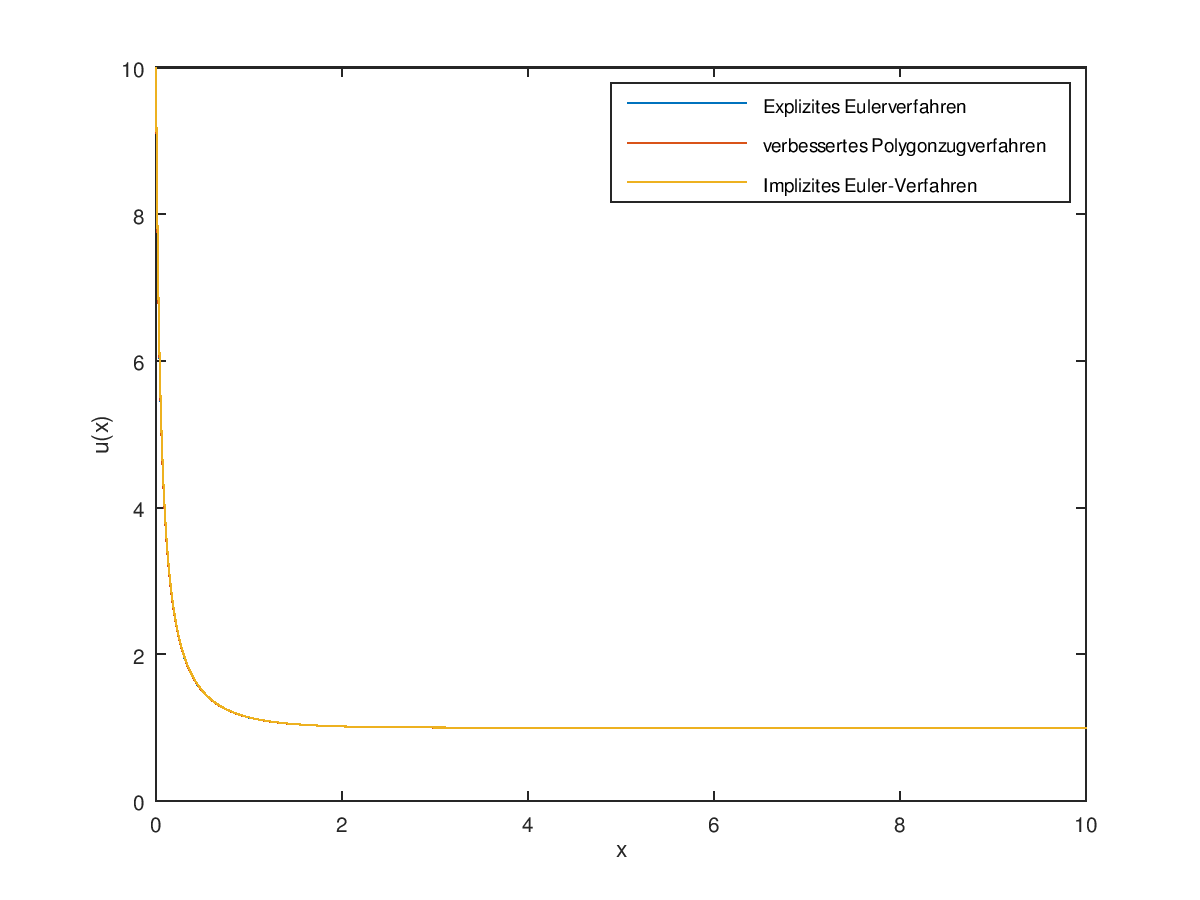
\includegraphics[width=.6\textwidth]{./loesung1.png}
    	\captionof{figure}{Numerische Lösung des Anfangswertproblems \eqref{aw1}}
    	\label{fig: loesung}
    \end{center}
    
    Betrachten wir hier schon einmal die Näherung in der Stelle $x=10$. Dabei wir jeder Schrittweite $h_i \defeq \frac{1}{100} * 0.5^{i-1}$ die entsprechende Näherung $u_{h_i}(10)$ zugeordnet.
    
    {
    	\centering
    	\begin{tabu}{l|l|l|l}
	    	\toprule
	    	\head $i$ & $u_{h_i}(10)$ Euler explizit & $u_{h_i}(10)$ Polygonzug & $u_{h_i}(10)$ Euler implizit\\
	    	\midrule \midrule
	    	0 & 1.0000000014427488 & 1.0000000018612263 & 1.0000001083003349 \\
	    	1 & 1.000000001638212  & 1.0000000018565394 & 1.0000000182649336 \\
	    	2 & 1.0000000017438231 &  1.0000000018554076 & 1.0000000063144361 \\
	    	3 & 1.0000000017987125 & 1.0000000018551316 & 1.0000000035060665 \\
	    	4 & 1.0000000018266939 & 1.0000000018550623 & 1.0000000025675782 \\
	    	5 & 1.0000000018408197 & 1.0000000018550432 & 1.0000000021864111 \\
	    	6 & 1.0000000018479125 & 1.0000000018550437 & 1.0000000020148434 \\
	    	7 & 1.0000000018514767 & 1.000000001855037 & 1.00000000193549 \\
	    	\bottomrule
	    \end{tabu}
		\captionof{table}{Näherunglösungfür  \eqref{aw1}}
		\label{tab: expeu_1}
    }

	\smallskip

	Zum Vergleich noch einmal die exakte Lösungen: $u_1(10) \approx 1,00000000185503826363587$.
	
	Für das Anfangswertproblem \eqref{aw2} verwenden wir ebenso das explizite Eulerverfahren und das verbesserte Polygonzugverfahren mit einer Anfangsschrittweite von $h=2$, die dann in $7$ Schritten jeweils halbiert wird. Damit ergibt sich das Bild der numerischen Lösung in \cref{fig: loesung2}.
	
	\begin{center}
		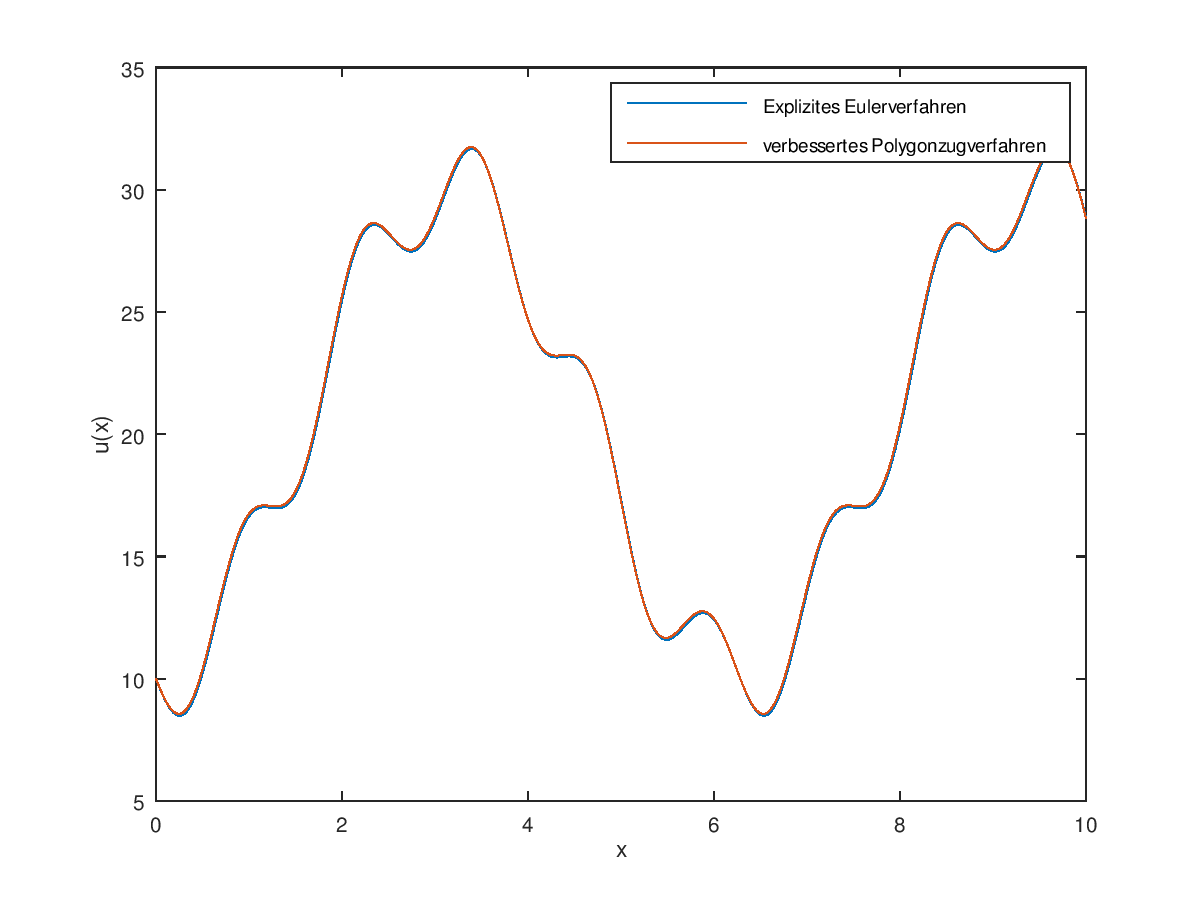
\includegraphics[width=.65\textwidth]{./loesung2.png}
		\captionof{figure}{Numerische Lösung des Anfangswertproblems \eqref{aw2}}
		\label{fig: loesung2}
	\end{center}

	Auch hier seien die Näherung für den Wert $u(10)$ bereits erwähnt. Erneut ordnen wir jeder Schrittweite $h_i \defeq \frac{1}{100} * 0.5^{i-1}$ die entsprechende Näherung $u_{h_i}(10)$ z.
	\begin{center}
		\begin{tabu}{l|l|l}
			\toprule
			\head $i$ & $u_{h_i}(10)$ Euler explizit & $u_{h_i}(10)$ Polygonzug\\
			\midrule \midrule
			0 & 15.942532391769284 & 2.6172434568951584 \\
			1 & 22.530915535595341 & 14.631286724808701 \\
			2 & 26.951452035021134 & 23.090920578941571 \\
			3 & 28.113171157763215 & 26.588114788175627 \\
			4 & 28.556201604193728 & 27.997347990269034 \\
			5 & 28.746142175550531 & 28.525781863185799 \\
			6 & 28.833371052366854 & 28.738458644584565 \\
			7 & 28.875059287667515 & 28.831446857490462 \\
			\bottomrule
		\end{tabu}
		\captionof{table}{Näherungslösung für \eqref{aw2}}
		\label{tab: expeu_2}
	\end{center}
	Zum Vergleich beträgt die exakte Lösung $u(10) = 28.915$

	\section{Fehlerbetrachtung}
	
	\begin{center}
		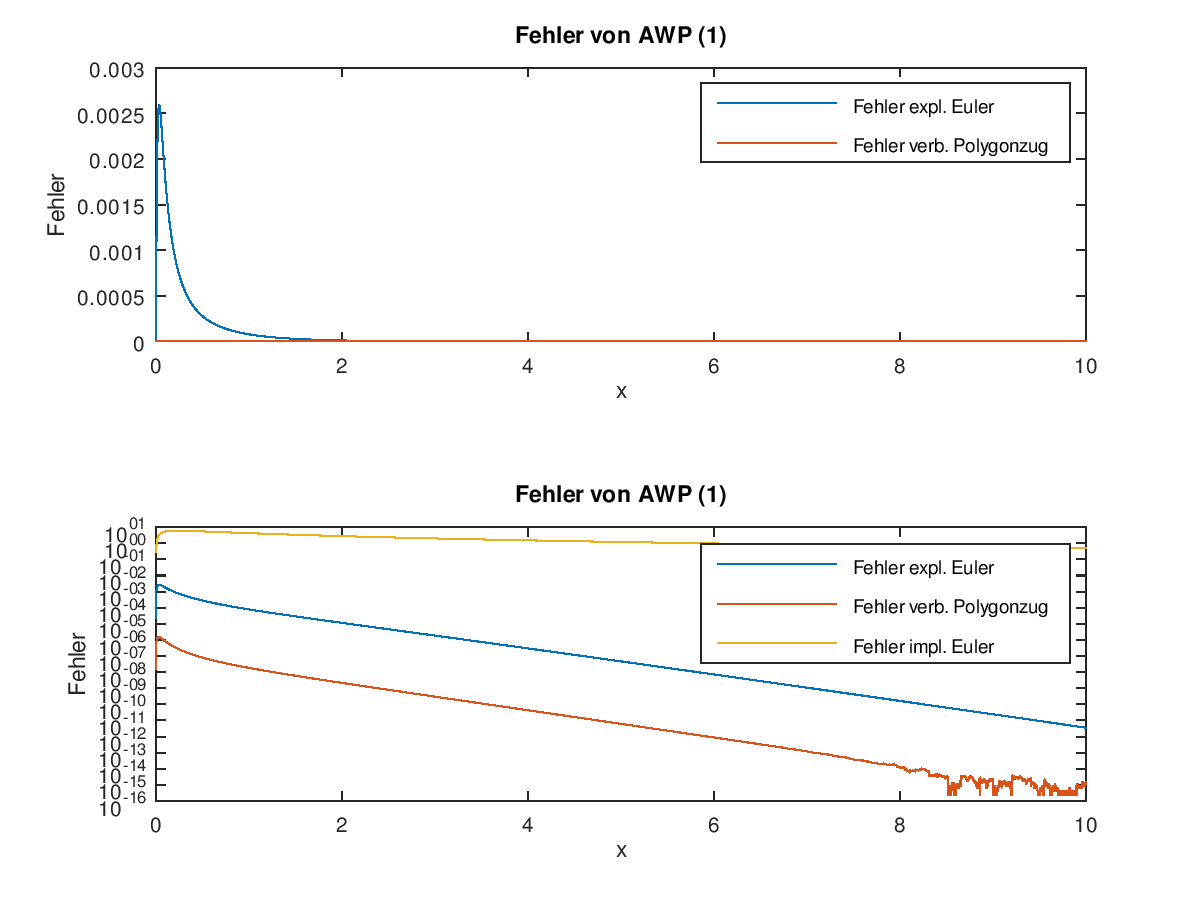
\includegraphics[width=.75\textwidth]{./fehler1.png}
		\captionof{figure}{Fehler in der Näherungslösung des AWP \eqref{aw1}}
		\label{fig: fehler1}
	\end{center}

	\begin{center}
		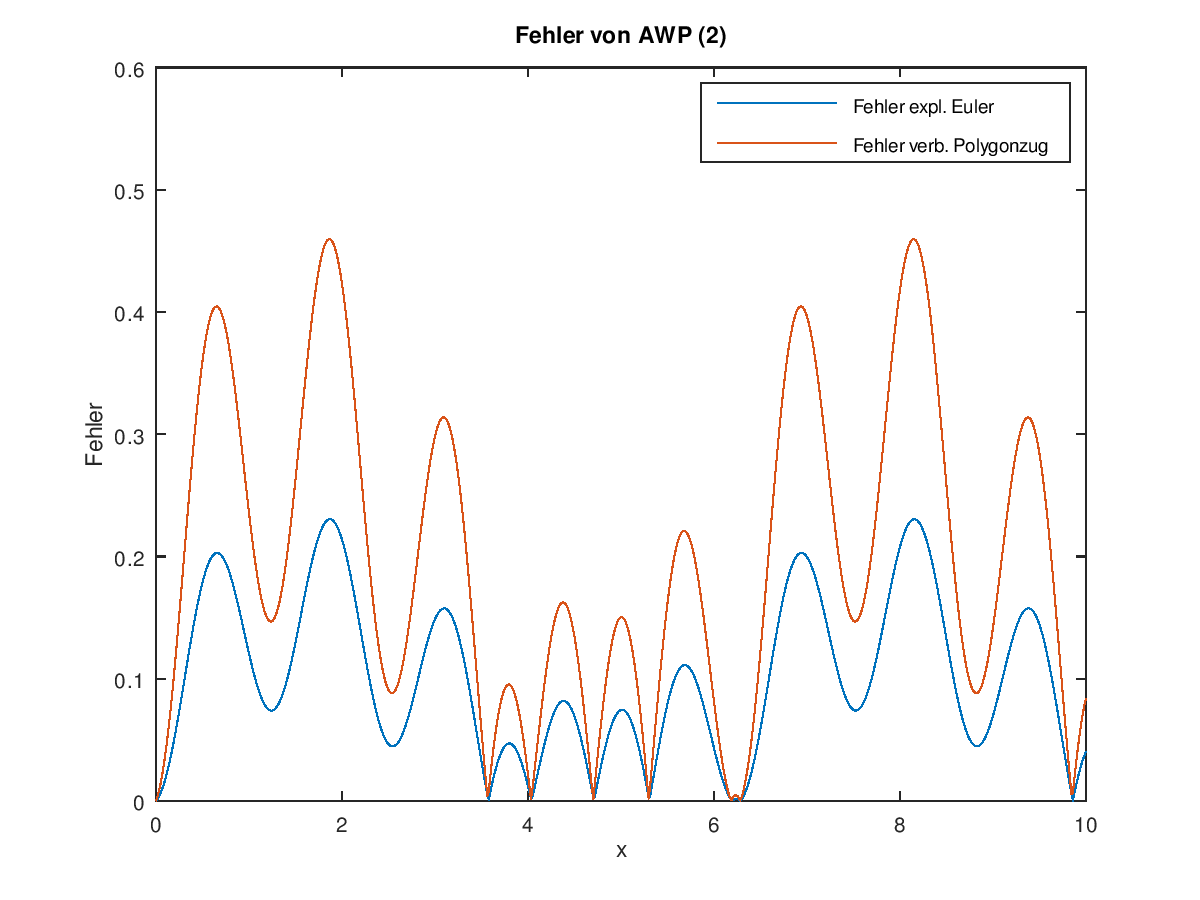
\includegraphics[width=.75\textwidth]{./fehler2.png}
		\captionof{figure}{Fehler in der Näherungslösung des AWP \eqref{aw2}}
		\label{fig: fehler2}
	\end{center}
	
	
	Wir berechnen die experimentelle Konvergenzordnung $\mathrm{EOC}(h_{N_1}, h_{N_2})$, wobei $h_i \defeq \frac{1}{100} * 0.5^{i-1}$.
	
	\smallskip
	
	\begin{center}
		\begin{tabu}{l|l|l|l}
			\toprule
			\head $i$ & Euler explizit & Polygonzug & Euler implizit \\
			\midrule \midrule 
			0 & 0.92711785521996615 & 2.0435143167844134 & 2.4979817240564346 \\
			1 & 0.96318524424129315 & 2.0232350778822767 & 1.7824201383743983 \\
			2 & 0.98148609898967798 & 1.9853269356211445 & 1.3884848412381854 \\
			3 & 0.99073108198050697 & 1.9593580155026575 & 1.1912373511171221 \\
			4 & 0.99528357306620763 & 2.2954558835261714 & 1.0943838138638462 \\
			5 & 0.99664696093629146 & 2.1255308820838581 & 1.047256320826385  \\
			6 & 1.0005395605775844  & 1.9999999999999951 & 0.98473008390473871 \\          
			\bottomrule
		\end{tabu}
		\captionof{table}{Experimentelle Konvergenzordnung für AWP \eqref{aw1}}
	\end{center}	
	
	\smallskip
	
	
	\begin{center}
		\begin{tabu}{l|l|l}
			\toprule
			\head $i$ & Euler explizit & Polygonzug \\
			\midrule \midrule 
			0 & 1.0228479237946984 & 0.8805471936163225 \\
			1 & 1.700780365142474  & 1.2942009292463943 \\
			2 & 1.2916018258023403 & 1.3234568924745176 \\
			3 & 1.1590887771215856 & 1.3419383854865135 \\
			4 & 1.0852655001393778 & 1.2363765324725053 \\
			5 & 1.0444287073921383 & 1.1385003484406608 \\
			6 & 1.0227166290239404 & 1.0750283818189208 \\          
			\bottomrule 
		\end{tabu}
		\captionof{table}{Experimentelle Konvergenzordnung für AWP \eqref{aw2}}
	\end{center}
	
	Für das Anfangswertproblem \eqref{aw1} ist anhand von \cref{fig: fehler1} erkennbar, dass das verbesserte Polygonzugverfahren einen geringeren Fehler aufweist als das explizite Eulerverfahren. Außerdem ist eine ungefähr doppelt so große experimentelle Konvergenzordnung zu erkennen. Damit konvergiert also das verbesserte Polygonzugverfahren schneller gegen die exakte Lösung. Das implizite Eulerverfahren dagegen weißt einen deutlich größeren Fehler auf als die beiden anderen Verfahren (man beachte allerdings die gröbere Schrittweite).

	Betrachten wir das Anfangswertproblem \eqref{aw2}. Es ist aus \cref{fig: fehler2} ersichtlich, dass hier das explizite Eulerverfahren einen geringeren Fehler als das verbesserte Polygonzugverfahren aufweist. Somit lässt sich also schließen, dass die Aufgabe \eqref{aw2} schlechter für das verbesserte Polygonzugverfahren geeignet ist als \eqref{aw1}. Dies spiegelt sich auch in der experimentellen Konvergenzordnung wieder, die beim expliziten Eulerverfahren im Vergleich zu \eqref{aw1} ungefähr gleich geblieben ist (bzw. leicht gestiegen). Das Polygonzugverfahren für \eqref{aw2} konvergiert hingegen nur ungefähr halb so schnell wie für \eqref{aw1} und damit ungefähr genauso schnell wie das explizite Eulerverfahren.
	
\end{document}
       